\documentclass[
    %paper = A4,		% Blattgröße
    11pt, 			% Schriftgröße	
    %DIV=12, 		% Satzspiegel
    %parskip=half,	% Absatzabstand
]{article}

%Seitenlayout
\usepackage{geometry}
\geometry{
   %left=2cm,
   textwidth=15cm,
   %top=2.5cm,
   bottom=3cm,
   %marginpar=10cm
   }

\usepackage[utf8]{inputenc}	% Dateicodierung
\usepackage[T1]{fontenc}	% Schriftcodierung
\usepackage[ngerman]{babel}	% Spracheinstellung

% Schriften
\renewcommand{\familydefault}{\sfdefault}
\usepackage{lmodern}		% Vektorschrift
\usepackage{microtype}		% keine Trennstrichen im Blocksastz


% Bilder
\usepackage{graphicx}
\graphicspath{{figures/}}
\usepackage{caption}

% Referenzbearbeitung
\usepackage{csquotes}
\usepackage[
	backend = biber,
	style = ieee        % ISO 690
    %style = authoryear-ibid %, maxcitenames=1, sorting=nyt  % Harvard 
	]{biblatex}
\addbibresource{literature.bib}

% Referenzbearbeitung Bildquellen
\newcommand*{\quelle}[1]{\par\raggedleft\footnotesize Quelle:~#1}

% Referenzierungen 
% immer als letztes einbinden
\usepackage[
	colorlinks = true,
	linkcolor = blue,
	citecolor = blue,
	%hidelinks,  % remove colouring
	]{hyperref}

\usepackage{blindtext}


\title{Blockchain- und IoT-Integration für die Revolution im Finanzsektor}
\author{Helena Stevanovic}
\date{08. April 2025}



\begin{document}
    \pagestyle{plain}
    \maketitle
    \thispagestyle{empty}


    \newpage
    \tableofcontents

    \section{Einleitung}

% und großer Dank an ChatGPT




Trotz gro\ss er technologischer Entwicklungen sind viele Bereiche im aktuellen Finanzsektor immernoch 
ineffizient.
In der traditionellen Bankenwelt ist das manuelle Abwickeln verschiedener 
Prozesse noch weit verbreitet und einer der Hauptgründe für die Ineffizienz. 
Von der Unterschrift auf einem Vertrag bis hin zur Veranlassung einer 
Überweisung - alle diese Prozesse erfordern Zeit und entsprechende Sorgfalt. Insbesondere die langsame 
Abwicklung von Verträgen und Zahlungen wirkt sich auf die Kundenzufriedenheit und die Wirtschaftlichkeit 
aus. Darüber hinaus stellt der Mensch als Fehlerquelle stets ein zusätzliches Risiko dar, das zu 
Verzögerungen und möglichen Kosten führen kann.

Heutzutage sind Banken- und mobile Bezahlsysteme wie Paypal in erster Linie zentral strukturiert, was 
bedeutet, dass das Vertrauen der Kunden in diese dritten Anbieter von entscheidender Bedeutung ist, 
insbesondere in Bezug auf die Datensicherheit. Des Weiteren stellt ein zentraler Knotenpunkt, in welchem
zwangsweise alle Datenflüsse zusammenflie\ss en und sich sämtliche Daten konzentrieren, ein attraktives 
Ziel für Cyberangriffe dar. Zusätzlich werfen unbekannte Datenflüsse und Funktionsweisen weitere 
Sicherheitsbedenken auf.


Die Revolutionierung traditioneller Finanzdienstleistungen durch innovative Technologien wie 
Blockchain und IoT öffnet Türen für eine Fülle von Möglichkeiten zur Effizienz- und Transparenzsteigerung.
%Auf der Suche nach Lösungen für diese Probleme zeigt die Kombination aus Blockchain-Technologie und 
%Internet der Dinge (IoT) ein enormes Potenzial. 
Die Blockchain kann die Automatisierung und Effizienzsteigerung der Prozesse ermöglichen und zudem durch
die Dezentralisierung viele Probleme von zentralisierten Systemen vermeiden. Währenddessen sorgt das IoT
für die Erhebung von Echtzeitdaten und verteilt diese im Netzwerk.
% nye
Trotz des vielversprechenden Potenzials, das diese Technologien bieten, gibt es jedoch 
auch rechtliche Hürden, die Berücksichtigung finden müssen. Es wird spannend sein zu sehen, wie sich 
Technologie und Gesetzgebung gemeinsam entwickeln, um den Finanzsektor effizienter, sicherer und 
kundenfreundlicher zu gestalten. Darüber hinaus wird der Umweltaspekt berücksichtigt und 
nach Möglichkeiten zur Verbesserung der Nachhaltigkeit gesucht.

% Erneuerbare



% Blockchain hat neue Möglichkeiten für Kleinanleger / private Anleger mit sich gebracht.

% Industrie 4.0 wird immer relevanter um die Effizienz zu steigern, Prozesse zu Optimieren
% und weltweit konkurrenzfähig zu bleiben.

% Außerdem bieten sich neue Möglichkeiten um die Wirtschaft zu globaliesieren(?)  Lieferketten\dots 

% Einsatzgebiete für eine praktikable Integration von BC und IoT im Finanzsektor aufgezeigt. 
% Die bereits in der Praxis angewendet werden oder existierende Prozesse optimieren können.
    \section{Blockchain}
In diesem Kapitel wird auf die revolutionären Vorteile der Blockchain 
eingegangen, durch die diese Technologie Einzug in den Finanzsektor gewonnen 
hat. Dem werden im Nachgang die einhergehenden Nachteile und Risiken gegenübergestellt. 

\subsection{Aufbau einer Blockchain}
Ein elementarer Grundbaustein einer Blockchain ist die Bildung eines Hashes.
\glqq Eine Hash-Funktion bildet eine beliebig große Menge an Eingabedaten [...] auf eine Zahl von 
fixer Größe ab, den sogenannten Hashwert\grqq{} \cite[p.~6]{fill2020blockchain}.
Die Hash-Funktion soll darüber hinaus drei wichtige Eigenschaften besitzen.
Das Diffusionsprinzip beschreibt eine deutliche Änderung des Hashwertes bei einem leicht
abgeänderten Eingabewert. Dadurch können unterschiedliche Eingaben sofort erkannt werden.
Das Konfusionsprinzip beschreibt die Eigenschaft, dass vom Hashwert nicht auf den Eingabewert
geschlossen werden kann. Beim Vergleich zweier Hashwerte von Eingaben mit einer minimalen
Änderung kann nichtmal auf die Position der Abweichung geschlossen werden.
Zuletzt ist die Kollisionsresistenz insbesondere im Bereich der Kryptographie relevant.
Eine Kollision tritt dann auf, wenn zwei unterschiedliche Eingaben auf denselben Hash abgebildet
werden. // Die Hash-Funktion soll hierfür möglichst vermeiden zwei unterschiedliche Eingabewerte
auf denselben Hashwert abzubilden.
\cite[p.~6ff]{fill2020blockchain} 

Um die Einsatzgebiete für eine Blockchain im Finanzsektor besser zu verstehen,
wird im Folgenden der Aufbau und die Komponenten grob dargestellt.
Im Block 1 wird zuerst jeweils ein Hash H1 und H2 für die Datenpunkte Transaktion 1 
und Transaktion 2 gebildet. Aus diesen Hashes wird dann ein gemeinsamer Hash H12 gebildet, 
der den Block Header 1 darstellt.
Analog zum Block Header 1 wird Block Header 2 erstellt. Zusätzlich enthält dieser eine
Referenz auf den vorigen Block Header 1 und ist somit der Kopf der Kette. Der Block Header 2
kann weiterführend im Block Haeder 3 eines dritten Blocks referenziert werden. 
\ref{fig:BC_Aufbau}
\cite[p.~17f]{fill2020blockchain}

\begin{figure}[h!]
    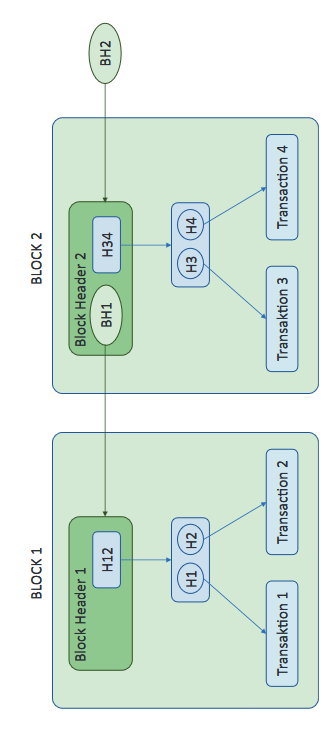
\includegraphics[width=\columnwidth]{BC_Aufbau.png}
    \quelle{\cite[p.~19]{fill2020blockchain}}
    \caption{Aufbau einer Blockchain \cite[p.~19]{fill2020blockchain}}
    \label{fig:BC_Aufbau}
\end{figure}


\subsection{Einsatzgebiete im Finanzsektor}
Bereits ... hat die Blockchain ihren Einzug in den Finanzsektor gefeiert. Manche
Sektoren sind aufgrund der Blockchain neu entstanden, wie der Kryptomarkt. Andere Sektoren,
wie der Aktienmarkt wurden dadurch grundlegend/stark verändert. Wieder andere Bereiche, in denen die Blockchain
einen essentiellen Teil bildet, sind nicht sehr bekannt. Im Folgenden wird der Einfluss
der Blockchain auf zuvor vorhandene Finanzsektoren, sowie neu erschlossene Sektoren 
betrachtet.

\subsubsection{Transaktionen / Kryptowährungen}
Der Kryptomarkt ist der wohl bekannteste Bereich, in der die Blockchain ein 
grundlegender Bestandteil ist. 
Die stärksten Kryptowährungen sind Bitcoin und Ethereum. 
Die Blockchain gewährleistet die Sicherheit und Nachvollziehbarkeit von Transaktionen.
\cite[p.~168]{chowdhary2025smart}
Das wird dadurch erreicht, indem die Transaktionen fest in der Blockchain codiert sind.
 \cite{}
% Verweis auf vorher verifizierte Blöcke & vollst. Kopie auf jedem teilnehmenden Gerät.
Die Blockchain-Technologie ermöglicht einen Peer-to-Peer Austausch von digitalen
Währungseinheiten. Dadurch werden Zwischeninstanzen, wie Banken und andere Zahlungsdienstleister,
die die Vertrauenswürdigkeit der Transaktionsakteure beglaubigen sollen, nicht benötigt.
\cite[p.~32]{fill2020blockchain}



\subsubsection{Tokenization von Assets}

\subsubsection{Smart Contracts}
\cite[p.~14]{pirafelnerblockchaintechnologie}

\subsubsection{Smart Grid im Energiesektor}
% Besser im Kapitel Nachhaltigkeit!
\cite[p.~72]{fill2020blockchain}


\subsection{Risiken bei der Integration von Blockshains}
\cite[p.~17]{pirafelnerblockchaintechnologie}
    \section{Fazit}

Eine Integration der Blockchain-Technologie bietet äußerst positive Möglichkeiten, um
Abläufe im Finanzsektor zu automatisieren und für alle Beteiligten zu optimieren.

Im Allgemeinen bietet der Aufbau einer Blockchain eine koherente Nachvollziehbarkeit aller 
Transaktionen und sichert die Integrität und Korrektheit der Daten. 
Aufgrund dessen kann sie eine Alternative für die Finanzbuchhaltung darstellen und bietet 
einen Schutz vor Bilanzfälschungen, da sonst die Integrität nicht gegeben wäre.
Des Weiteren sorgt die Dezentralisierung der Blockchain für eine hohe Robustheit und 
Transparenz der Systeme.
Ausfälle von einzelnen Rechnerknoten können ohne einen Mehraufwand von anderen Knoten
kompensiert werden und insgesamt kann auf zentrale Datenspeicher verzichtet werden.
\cite[p.~70]{fill2020blockchain}
Zudem sorgen die Eigenschaften eines Blockchain-basierten Systems dafür, dass es ein
unattraktiveres Ziel von Cyberangriffen wird und dadurch finanzielle Schäden verhindert
werden. Dies ist ein enormer Vorteil im Finanzsektor, da dieser immer ein lukratives Ziel 
für Hacker sein wird.
\newline
Die Nutzung von Smart Contracts sorgt für bemerkenswerte Effizienssteigerungen in
Geschäftsprozessen. 
Aufgrund der Transparenz durch definierte Abläufe in den Vertragsbestimmungen können 
rechtliche Streitigkeiten reduziert werden. Dadurch werden Unterbrechungen zur Klärung von
Rechtsfragen verringert und Anwaltskosten reduziert. Eine zeitliche Abschätzung von 
Geschäftsprozessen wird hierdurch planbarer.
Jedoch müssen die Vertragsbestimmungen vorab juristisch abgesichert sein, sodass der Smart 
Contract seine rechtliche Verbindlichkeit behält. Dies kann vor allem bei internationalen
Verträgen problematisch sein, da mehrere örtliche Regelungen berücksichtigt werden müssen.
Dieser Mehraufwand in der Vorbereitung ist lohnenswert, da sowohl Fehlerquellen, 
als auch Bearbeitungszeiten und Gebührenkosten verringert werden.
\newline
Die Blockchain ist demnach eine wünschenswerte Ergänzung im Finanzsektor, die als 
vertrauenswürdiger Dienst zentralisierte Systeme ersetzen kann.
Bei der Nutzung von bereits bestehenden Blockchains kann jedoch eine fehlende zentrale 
Instanz, die die Weiterentwicklung der Technologie koordiniert, für Probleme in der 
Abwärtskompatibilität sorgen. In dem Fall muss auf die Entwickler-Community vertraut werden,
wodurch keine Planungsstabilität gegeben ist.
\cite[p.~70f]{fill2020blockchain}










Darüber hinaus ist die Kritik an der Nachhaltigkeit der Ressourcenverwendung in 
Blockchain-Technologien hervorzuheben. Verschiedene Konsensalgorithmen wie Proof-of-Stake 
oder Proof-of-Energy-Efficiency können jedoch zur Reduzierung des Energieverbrauchs 
beitragen. 
\newline
Insgesamt bietet die Blockchain-Technologie dem Finanzsektor und darüber hinaus bedeutende 
Vorteile, verlangt jedoch nach einem verantwortungsbewussten Umgang mit Datensicherheit, 
Datenschutz und Energieverbrauch.

    \printbibliography
    \listoffigures
\end{document}